\documentclass[xcolor=table]{beamer}
\usepackage[utf8]{inputenc}
\usepackage[T1]{fontenc} 
\usepackage[english]{babel} 
\usepackage{graphicx}
\usepackage{comment}
\usepackage{graphicx,wrapfig,lipsum}
\usepackage{hyperref}
\usepackage{tcolorbox}
\hypersetup{
    colorlinks=true,
    linkcolor=blue,
    filecolor=magenta,      
    urlcolor=cyan,
}
\setbeamertemplate{footline}[text line]{%
  \parbox{\linewidth}{\vspace*{-8pt}\today\hfill\insertshortauthor\hfill\insertpagenumber}}{}

%%Defining the ``proposition'' environment
\newtheorem{proposition}{Proposition} 

%%Sets the beamer theme "Cuerna"
\usetheme{Cuerna} 

\usecolortheme{default}
%Available color themes: default, bluesimplex, brick, lettuce

%%Insert the logo
\logo{
\includegraphics[width=1.7cm]{plots/logo.jpeg}}

%%Title
\title{TELLIE PCA:\\ Processing \\ Automation}

\author{Michal Rigan\\ %Author
          \texttt{mrigan@snolab.ca}} %e-mail
          
\date{\textbf{Report}\\
\today} %Date or event

\institute{University of Sussex} %%Institution

\begin{document}

{
\setbeamertemplate{footline}{} 
\begin{frame}
  \titlepage %Creates the title page
\end{frame}
}

\begin{frame}{Processing automation - Why}
\begin{itemize}
	\item extracting and validating PCA constants from data is complex...
	\item \textbf{Goal}: streamline (possibly speed up) the process of obtaining the PCA constants from data
	\begin{itemize}
		\item regardless of the method to obtain the data
		\item modular
		\item require minimum human input
		\item provide monitoring
	\end{itemize}
\end{itemize}
\end{frame}

\begin{frame}
\noindent\makebox[\textwidth]{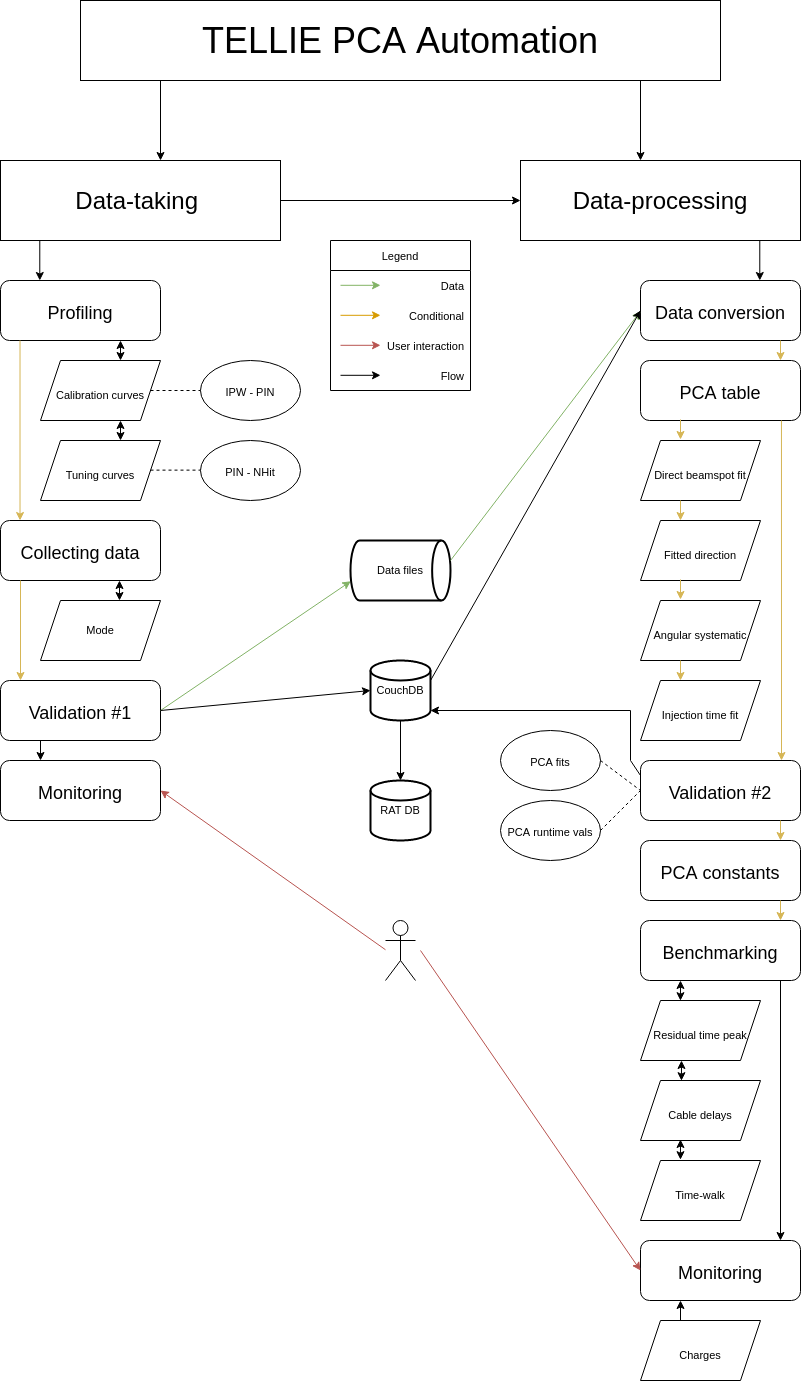
\includegraphics[width=0.491\textwidth]{plots/overview.png}}
\end{frame}

\begin{frame}{Processing automation - What}
\begin{itemize}
	\item \textit{validate \#1} $\rightarrow$ validates data is `good enough` for PCA $\rightarrow$
	\item \textit{PCA table} $\rightarrow$ fits for required corrections: beamspot fit, fibre direction, angular systematic, injection time
	\item \textit{PCA table} $\rightarrow$ compare these fits and runtime values to previous set (stability)
	\item \textit{validate \#2} $\rightarrow$  validates fits are `sensible`
	\item \textit{PCA constants} $\rightarrow$ extracts PCA constants (PCA processor)
	\item \textit{Benchmarking} $\rightarrow$ benchmarks the constants against previous set
	\item \textit{Monitoring} $\rightarrow$  provides monitoring of each step, and between datasets (!)
\end{itemize}
\end{frame}

\begin{frame}{Processing automation - Validations}
Run series of checks:
\begin{itemize}
	\item Validation \#1:
	\begin{itemize}
		\item correct fibre, number of events (EXTA), passed hits, cuts on PMTs, checks on LPC, run length, frequency
		\item NHit distribution, NHit over time, delays
		\item time of hits over time, \# peaks, PMTs in beamspot, PMT occupancy
		\item PIN, PIN vs NHit, events over subruns, ... (21 total)
	\end{itemize}
	\item Validation \#2:
		\begin{itemize}
		\item for each correction: check mean, rms, min, max 
		\item residual times: distribution, \# peaks, function of angle
		\item evaluate trends (12 total)
	\end{itemize}
	\item this is available on monitoring page (flags $\rightarrow$ bitword)
\end{itemize}
\end{frame}

\begin{frame}{Processing automation - Benchmarking}
\begin{itemize}
	\item compare PCA values (cable delays, TW fit) to previous set
	\item apply these constants to a well understood run
	\item extract the residual hit times distribution
	\item monitor charges: threshold, peak, hhp for QHS \& QHL
\end{itemize}
\end{frame}

\begin{frame}{Processing automation - How}
\begin{itemize}
	\item \textit{simple} $\rightarrow$ only requires to provide a runlist
	\item \textit{modular} $\rightarrow$ master script that spawns subprocesses, individual steps can be (re)run. Also allows for easier changes to modules
	\item \textit{submission platform} $\rightarrow$ can queue processes, submit (up to a limit), monitor their status
	\item \textit{customizable} $\rightarrow$ thresholds (other settings) are loaded from environment (tuning)
	\item \textit{linked} $\rightarrow$ stores data in couchdb, ratdb, redis, provides plots to minard
	\item \textit{regulation} $\rightarrow$ unifies cuts, data checks, event selection, ranges, ...
	\item \textit{evaluative} $\rightarrow$ provides bitwords (flags) for fits / checks
\end{itemize}
\end{frame}

\begin{frame}{Processing automation - Minard}
\noindent\makebox[\textwidth]{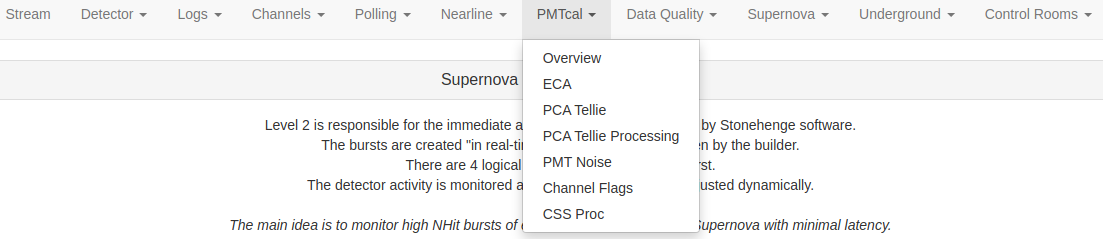
\includegraphics[width=1\textwidth]{plots/1.png}}
\end{frame}

\begin{frame}{Open questions}
\begin{itemize}
	\item tagging events outside Orca
	\item when (from) to apply new constants
	\item ensure recent ECA
	\item where to deploy
	\item data-taking (modes) implementation (\href{https://www.snolab.ca/snoplus/private/DocDB/cgi/ShowDocument?docid=7612}{\#7612})
\end{itemize}
\end{frame}

\begin{frame}{Processing automation - Next steps}
\begin{itemize}
	\item documentation
	\item minard PR
	\item help to deploy
	\item ...
	\item tuning of the threshold values
	\item PR for PCA Proc
\end{itemize}
\end{frame}

\end{document}